\documentclass[11pt,a4paper]{article}

\usepackage[margin=1in]{geometry}
\usepackage{amsmath,amssymb}
\usepackage{graphicx}
\usepackage{booktabs}
\usepackage{xcolor}
\usepackage{caption}
\usepackage{microtype}

\captionsetup{font=small,labelfont={bf},labelsep=period}
\emergencystretch=1.2em
\usepackage[colorlinks=true,linkcolor=red!60!black,citecolor=green!45!black,urlcolor=blue!60!black]{hyperref}
\usepackage{xurl}

\newcommand{\dex}{\ensuremath{\,\mathrm{dex}}}

\title{\textbf{The price of absolute scale: degeneracy groups, surviving\\ statistics, and the reference economics of cellular signalling}}
\author{Huan Li\\[2pt]
\small Shanghai Liangta Biotech Co., Ltd., Shanghai 201899, China\\
\small Correspondence: hl@liangtabio.com\quad ORCID: 0009-0004-2695-6825}
\date{}

\begin{document}
\maketitle

\begin{abstract}
\noindent
A cell that senses its environment must do so with instruments it cannot calibrate: every molecular gain in a signalling pathway drifts, and no external standard exists inside a cell. Which statistics of an input can survive transmission through such pathways, and what must a cell pay to report anything absolute? We formalise the question by attaching to each pathway layer its degeneracy group, the parameter transformations that leave the output distribution invariant, and we define the survival set of statistics that cross the layer unchanged. For the generic affine interface the survival set is computable and sharp: difference ratios, signs, counts and event times survive unconditionally; amplitude survives only where the gain is pinned from outside; fold change survives only where the basal term vanishes. Cascades compose under an exact information-loss identity that decomposes the total loss across layers and identifies the largest single loss. References fall into three classes: calibration-free statistics (class I), structural constants maintained by physics (class II), and paid references maintained by active feedback at continuing cost (class III), the last diagnosable by three operational markers. The resulting principle, that class-III payment arises where function references absolute scale, is tested on four worked instances with new analyses of public data: the covalent-modification cycle (six physical parameters collapse to two identifiable combinations, with an exact Fisher zero direction on absolute scale and an interior information optimum away from the zero-order limit); the Bicoid morphogen anchor, which is absolute yet free because physics fixes its length constant (scaling exponent $-0.18$, 95\% CI $[-0.48, 0.11]$, 581 embryos, exact scaling excluded at $8.3\sigma$), while embryonic scaling is supplied by nuclear counting; Wnt fold-change readout, quantised to a plateau within $\pm5\%$ between 7 and 49 mM LiCl with the breakdown bracketed between 48.6 and 58.1 mM; and two signalling cascades in which absolute amplitude dies in the across-cell gain distribution while self-referenced statistics survive. A positive control in yeast osmotic homeostasis fires all three class-III markers, and causal inhibition of the maintenance loop abolishes absolute-scale recovery (0.644 to 0.070). Every prediction was registered before the corresponding data were inspected; the record across sixteen clauses is eight confirmations (four with registered contractions), six falsifications, and two clauses awaiting data. Scale-free statistics are not a style of signalling; they are the only currency that survives the cell's own gauge freedom.
\end{abstract}

\section{Introduction}

Quantitative cell biology has accumulated two bodies of fact that sit uncomfortably apart. The information-theoretic literature measures how much information flows through biochemical circuits and what architectures optimise the flow \cite{Tkacik2025,Cheong2011,Selimkhanov2014,Bowsher2014,Govern2014}. The parameter-inference literature documents that behaviour underdetermines parameters: fits are sloppy, and widely different molecular parameter sets produce identical behaviour \cite{Gutenkunst2007,Prinz2004,Goaillard2021}. What neither literature answers is the complementary question a cell itself must solve: given that its own parameters are not observable from its own behaviour, which statistics of its input can it even report downstream? A pathway is, from the inside, an instrument whose calibration it can never check.

This paper turns that observation into a computable object. The tool is the degeneracy group of a pathway layer: the set of parameter transformations that leave the output distribution invariant for every input. Two parameter values on one orbit of this group cannot be distinguished from the output at any measurement precision, so the group's orbit invariants are exactly what a downstream layer can receive. Everything else is gauge. The same mathematical object has appeared on the assay side of measurement science, where scale degeneracy makes analytical assays uncalibratable and forces counting-based readouts \cite{Guo2026,Vogelstein1999}; here it is applied inside the cell.

Three questions organise the paper. First, structure: which input statistics survive a layer, and which die? Second, composition: what survives a cascade of layers? Third, economics: when a function genuinely requires an absolute quantity, what does the cell pay, and where? The answers are, respectively, a computable survival set with a sharp algebraic content; an exact information-loss identity that decomposes the loss across layers; and a three-class reference taxonomy with operational markers, from which a falsifiable principle follows: class-III payment arises where function demands absolute scale. The converse is tested rather than assumed, and the one class-II anchor in the record (the Bicoid length constant) is the case where it fails. Four worked instances on public data supply the empirical content, and a companion series applies the same machinery at full depth to three systems that this paper only summarises: the p53 pulse encoder \cite{CompanionP53}, the bacterial chemotaxis receptor layer \cite{CompanionChemo}, and the field-level pharmacology of GPCR bias \cite{CompanionGPCR}.

The thesis is narrow and falsifiable. Cellular communication is implemented, wherever the record allows the test, in statistics invariant under the multiplicative-scale degeneracy group of the intracellular environment, because nothing else is reportable across it. Where the claim fails, the failure is recorded in the same ledger as the confirmations (Table~\ref{tab:ledger}).

\section{The model: layers, degeneracy groups, survival sets}
\label{sec:model}

\subsection{Layers and the degeneracy group}

The input is a stochastic process $S(t)$ drawn from an ensemble with distribution $p_S$. An input statistic $X=f(S)$ (a difference ratio, a sign, a count, an event time, an amplitude) is defined independently of layer parameters. Layer $i$ is a stochastic map: given its upstream input and parameters $\theta_i\in\Theta_i$, its output symbol is distributed as $Y_i\sim P(Y_i\mid\text{upstream},\theta_i)$, with biochemical noise absorbed into $P$. A cascade is a Markov chain $L_1\to\cdots\to L_n$, $Y_0=S$. The degeneracy group of layer $i$ is the group of parameter transformations leaving the output distribution invariant:
\begin{equation}
G_i=\Big\{\,g:\Theta_i\to\Theta_i\ \Big|\ P(Y_i\mid Y_{i-1},\theta)=P(Y_i\mid Y_{i-1},g\cdot\theta)\ \ \forall\,Y_{i-1},Y_i\,\Big\}.
\label{eq:group}
\end{equation}
The identifiable content of the layer is exactly the set of orbit invariants of $G_i$. Layers are delimited by information structure rather than biochemical topology: parameters unidentifiable from the same output belong to one layer, and a feedback parameter is assigned to the layer from whose output it is unidentifiable. Under this assignment, cross-layer feedback (adaptation canonically) is absorbed into a single layer and the Markov property is retained (Fig.~\ref{fig:schematic}a).

\subsection{The survival set}

Let $a_i$ be the transmitted readout functional of layer $i$, the alphabet map the downstream layer consumes. With $\Theta_i^{\mathrm{work}}$ the physiological working range and $\varepsilon$ calibrated to the system noise level, the survival set is
\begin{equation}
T_i=\Big\{\,X:\ \sup_{\theta\in\Theta_i^{\mathrm{work}},\,g\in G_i}\ \mathrm{TV}\Big(P\big(a_i(Y_i)\mid X,\theta\big),\,P\big(a_i(Y_i)\mid X,g\cdot\theta\big)\Big)<\varepsilon\,\Big\},
\label{eq:survival}
\end{equation}
where $\mathrm{TV}$ is total variation. Two features of the definition carry weight. The condition acts on the distribution of the readout $a_i(Y_i)$, not on the raw output distribution; acting on the raw output, any unidentifiable gain (the generic case) makes every output sensitive to $g$ and the survival set is identically empty. And the operative source of gain degeneracy is joint confounding: with channel gain $k$ and input ensemble both unknown, $(k,p_X)$ and $(ck,p_{X/c})$ induce identical output distributions, so the degeneracy lives in the input-ensemble direction, of which (\ref{eq:survival}) is the operational projection.

\subsection{Interface algebra: what survives}
\label{sec:algebra}

Which statistics survive depends on the function class of the interface. The generic biological interface is affine, $y=kx+b$, with $b$ a basal term (spontaneous activation, basal expression, leak) and the gain $k$ generically unidentifiable. Direct substitution gives the survival table. Fold change does not survive: in $(kx_1+b)/(kx_0+b)$ neither $k$ nor $b$ cancels, and fold survives only at $b=0$. Difference ratios survive: $(y_3-y_2)/(y_2-y_1)=(x_3-x_2)/(x_2-x_1)$, with $k$ and $b$ both cancelling. The sign survives for $k>0$. Counts and event times survive because threshold-crossing order and timing are affine-invariant. Amplitude survives if and only if the gain is pinned from outside; an increment survives where ratios survive and the gain is pinned to the precision the downstream consumer requires. The generic survival set is therefore $\{\text{sign, increment, difference ratio, count, event time}\}$, and the fold-change literature \cite{Goentoro2009iFFL,Shoval2010,Adler2018} describes the special case $b\approx0$ or an actively normalised interface (Fig.~\ref{fig:schematic}b). Adaptation has a compact identity in this algebra: an adaptor actively subtracts the baseline and thereby pulls the affine interface back onto the increment channel. What adaptation purchases is the survival of the difference family.

\subsection{The three-leg criterion}

A statistic $X$ crosses interface $\varphi_i$ if and only if three conditions hold simultaneously (Fig.~\ref{fig:schematic}c). Leg 1, algebraic survival: $X\in T_i$ in the sense of (\ref{eq:survival}); the failure mode is scale leak. Leg 2, symbolic reachability: $I(X;Y_i)>0$; the failure mode is an invariant but uninformative statistic. Leg 3, temporal bandwidth: the statistic's timescale lies inside the interface's perturbation--response bandwidth, defined in the time domain by modulating the input at timescale $\tau$ and recording whether the output response stands above the noise floor; the failure mode is erasure by filtering.

\subsection{The information-loss identity}

Cascades compose exactly. For the Markov chain $S\to Y_1\to\cdots\to Y_n$, define the loss at layer $i$ as $L_i=I(S;Y_{i-1})-I(S;Y_i)$, with $Y_0=S$.

\begin{quote}
\textbf{Theorem 1 (information-loss identity).} $H(S)=I(S;Y_n)+\sum_{i=1}^{n}L_i$, and mutual information is monotone, $I(S;Y_1)\ge\cdots\ge I(S;Y_n)\ge0$. The weakest layer $i^*=\arg\max_i L_i$ carries the largest loss of input information, and for any statistic $X=f(S)$ the per-statistic chain $I(X;Y_1)\ge\cdots\ge I(X;Y_n)$ bounds end-to-end transferable content by the weakest-layer loss.
\end{quote}

\noindent The proof is telescoping plus the data-processing inequality. The identity needs no capacity concept and is bit-exact on numerical checks (Methods). Passing layer by layer is necessary but not sufficient end to end: the end-to-end survival set obeys $S_{\mathrm{cascade}}\subseteq T_1\cap\varphi_1^{-1}(T_2)\cap\cdots\cap T_n$, and the gap comes from loss of leg-2 sensitivity under composition and from alphabet re-quantisation. We state the bound as loose and use it only to locate where information dies.

The status of the framework is stated precisely. Theorem 1 is a theorem given the model; the survival set and the three-leg criterion are operational definitions; no tightness, reachability, or capacity claim is made.

\begin{figure}[p]
\centering
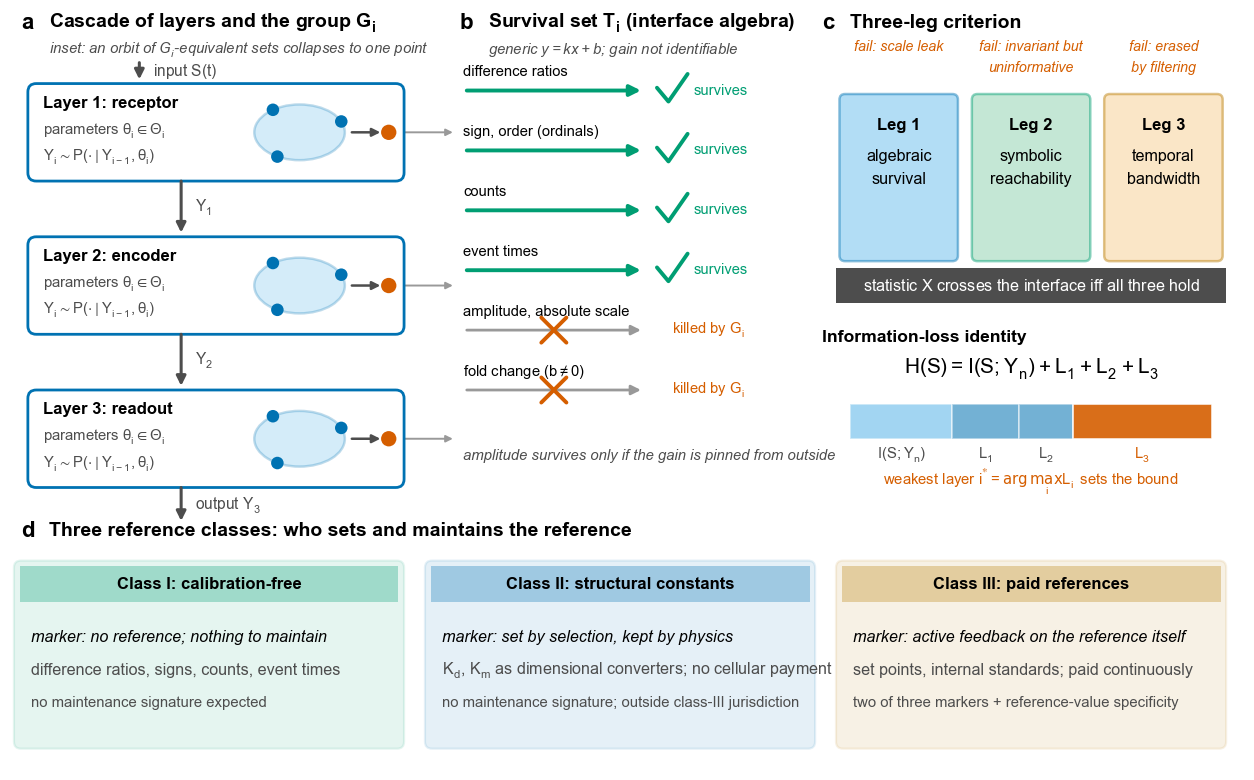
\includegraphics[width=\textwidth]{fig1_schematic.png}
\caption{The framework in one view. \textbf{a}, A pathway as a cascade of stochastic layers; the degeneracy group $G_i$ collapses each layer's parameter space onto an orbit, and only orbit invariants are reportable downstream. \textbf{b}, Interface algebra: for the generic affine interface $y=kx+b$ with unidentifiable gain, difference ratios, signs, counts and event times survive unconditionally; amplitude is killed by the group unless the gain is pinned from outside; fold change survives only where the basal term vanishes. \textbf{c}, The three-leg criterion: a statistic crosses an interface if and only if it survives algebraically, is symbolically reachable, and fits the temporal bandwidth. The information-loss identity decomposes input entropy into transmitted information plus per-layer losses, identifying where the largest single loss occurs. \textbf{d}, The three reference classes: calibration-free statistics, structural constants maintained by physics, and paid references maintained by active feedback.}
\label{fig:schematic}
\end{figure}

\section{The price of absolute scale: three reference classes}
\label{sec:payment}

The naive dichotomy, free scale-free statistics versus paid absolute quantities, has a hole: molecular constants such as $K_d$ and $K_m$ are absolute in units yet free of cellular maintenance, so a signature of the form ``wherever absolute scale is referenced there must be active maintenance'' would flag every $K_m$-driven reaction as a false positive. The classification axis is therefore not the object type but who sets and maintains the reference, and on what timescale (Table~\ref{tab:classes}, Fig.~\ref{fig:schematic}d).

\textbf{Class I, calibration-free statistics.} Difference ratios, signs, counts, event times. No reference is needed and nothing is maintained.

\textbf{Class II, structural constants.} $K_d$, $K_m$ and their dimensionless combinations: set by natural selection and maintained by physics (molecular structure). On signalling timescales the cell does not maintain them at a continuing cost, and they trigger no maintenance signature; they can nevertheless be retuned on longer timescales by expression, post-translational modification and evolution. They are dimensional converters mapping an external absolute concentration $[L]$ to the internal dimensionless occupancy $[L]/(K_d+[L])$.

\textbf{Class III, paid references.} Set points, internal standards, and physiologically regulated effective constants, such as the methylation-adjusted effective affinity of the chemotaxis receptor: set by the cell, maintained by active feedback, drifting if unmaintained, and paid for continuously.

A site is classified III when at least two of three operational markers hold, with reference-value specificity required: (1) negative feedback acts directly on the reference set point itself; (2) direct perturbation of the reference value is followed by recovery to the same set point (recovery of a downstream response does not count); (3) maintaining the reference consumes extra energy, and inhibiting the energy supply makes the reference drift. The markers are scored independently of the framework's own predictions, so a class-III assignment cannot be invoked after the fact to rescue a failed prediction. The payment position is the intersection of \{points where function references absolute scale\} with class III, determined by functional demand, not by where information is lost: a terminal decision referencing only relative quantities pays nothing; one referencing absolute position must establish and maintain a local reference there.

\begin{quote}
\textbf{Corollary (free-first principle).} Wherever a class-I statistic suffices for the function, it is the one used; class-III payment appears at the positions where function references absolute scale. \emph{Falsifiable form:} a single position whose function references only relative quantities yet which hosts an active, energy-consuming reference-maintenance mechanism falsifies this first half. The converse, that every function referencing absolute scale must pay, is not claimed as a universal: a class-II structural constant supplied by physics satisfies such a function without dedicated maintenance, and the Bicoid length constant of Section~\ref{sec:bicoid} is the instance in this record.
\end{quote}

Three prospective predictions follow, stated before the worked instances. For steady state $S_0$ and perturbation $\Delta S$, define absolute sensitivity $dY/dS_0$ and relative sensitivity $dY/d(S/S_0)$. \textbf{P-1 (deletion):} deleting a class-III maintenance mechanism predicts $dY/dS_0\to0$ with $dY/d(S/S_0)$ preserved; retained absolute sensitivity with no substitute maintenance falsifies. \textbf{P-2 (synthetic circuit):} a circuit with no active internal standard but passive structural constants predicts $dY/dS_0\approx0$ with nonzero relative sensitivity; stable absolute-scale transmission falsifies. \textbf{P-3 (search):} positions that functionally require absolute position but show no reported maintenance machinery form an exhaustive search list; a hit confirms, and an exhaustively documented absence triggers re-examination rather than a verdict against the framework, because ``not found'' and ``absent'' cannot be separated in practice.

\begin{table}[t]
\centering
\caption{The three reference classes. The classification axis is who sets and maintains the reference, on what timescale; class III is diagnosed by the three operational markers of Section~\ref{sec:payment}.}
\label{tab:classes}
\small
\begin{tabular}{@{}p{2.6cm}p{3.6cm}p{3.4cm}p{4.6cm}@{}}
\toprule
 & \textbf{Class I: calibration-free} & \textbf{Class II: structural constants} & \textbf{Class III: paid references} \\
\midrule
Objects & difference ratios, signs, counts, event times & $K_d$, $K_m$, dimensionless combinations & set points, internal standards, regulated effective constants \\
Set by & nobody & natural selection & the cell \\
Maintained by & nothing to maintain & physics (molecular structure) & active feedback, at continuing cost \\
If unmaintained & -- & invariant on physiological timescales & drifts \\
Maintenance signature & none & none (outside class-III jurisdiction) & feedback on the reference; recovery of the reference; drift on energy inhibition \\
\bottomrule
\end{tabular}
\end{table}

\section{Worked instance 1: the static sensor is blind to its own absolute scale}
\label{sec:pdpc}

The phosphorylation--dephosphorylation cycle (the Goldbeter--Koshland motif \cite{Goldbeter1981}) converts an input activity ratio into a steady-state modified fraction. With substrate total $S_T$, kinase and phosphatase maximum rates $V_1,V_2$, and modified fraction $u$, the symmetric-Michaelis steady state obeys
\begin{equation}
\xi=\frac{u}{1-u}\cdot\frac{\kappa+1-u}{\kappa+u},\qquad \xi\equiv\frac{V_1}{V_2},\quad \kappa\equiv\frac{K_m}{S_T}.
\label{eq:gk}
\end{equation}
The $\kappa\to0$ limit is the zero-order switch; $\kappa\to\infty$ degenerates to a graded Michaelian response.

\begin{quote}
\textbf{Theorem 2 (degeneracy group).} The steady-state dose--response curve of (\ref{eq:gk}) depends on the six physical parameters $(k_1,E_{1T},k_2,E_{2T},K_m,S_T)$ only through the two dimensionless combinations $(\xi,\kappa)$. The degeneracy group is four-dimensional, generated by the joint product rescalings of $k_1E_{1T}$ and of $k_2E_{2T}$, by $(K_m,S_T)\to(sK_m,sS_T)$, and by an independent enzyme-total direction. All absolute molecular scales are structurally unidentifiable from steady-state fitting.
\end{quote}

Four parameter sets differing in every individual parameter by up to five-fold produce steady-state curves identical to the last digit of double-precision arithmetic (max $|\Delta u|=0$ for the $(K_m,S_T)\times5$ action; $1.7\times10^{-18}$ for the rate--enzyme actions; Fig.~\ref{fig:pdpc}b). The asymmetric-Michaelis extension ($\kappa_1\neq\kappa_2$) raises the identifiable set to the triple $(\xi,\kappa_1,\kappa_2)$ and leaves the group four-dimensional: asymmetry enlarges the identifiable set, not the group. The local logit slope has the exact closed forms
\begin{equation}
n_H=1+\frac{1}{2\kappa}\qquad\text{(symmetric)},\qquad
n_H=\frac{4}{4-1/(\kappa_1+\tfrac12)-1/(\kappa_2+\tfrac12)}\qquad\text{(asymmetric)},
\label{eq:hill}
\end{equation}
agreeing with numerical logit slopes to relative deviations $\le7.2\times10^{-10}$ (symmetric case) and $\le1.1\times10^{-14}$ (asymmetric case). Asymmetry has a sign effect: at $\kappa_2=0.01$, an asymmetry ratio $r=\kappa_1/\kappa_2=0.03$ raises $n_H$ to $98.973$ while $r=30$ lowers it to $5.068$ (Fig.~\ref{fig:pdpcfull}d).

\begin{quote}
\textbf{Theorem 3 (Fisher barrier).} Under additive Gaussian measurement noise on a 20-point titration design spanning three decades ($\sigma=0.03$, Western-blot grade), the shape parameterisation $(\ln c,\ln\kappa)$ is well conditioned (condition number $\chi\approx19$--$33$ over $\kappa\in[0.005,1]$), while the absolute parameterisation $(\ln c,\ln K_m,\ln S_T)$ carries an exact zero eigenvalue along the group orbit. The barrier is structural: no increase in sample size or precision crosses it. In double precision that zero is returned as a numerical zero, so the absolute block's reported condition number measures the zero (of order $10^{33}$ at $\kappa=0.005$ and at $\kappa=0.5$ alike), not a finite measurement budget.
\end{quote}

Only an orthogonal measurement axis crosses the barrier: substrate titration moves $\kappa=K_m/S_T$ point by point while enzyme titration holds $\kappa$ fixed and moves $\xi$, and combining the two converts absolute $K_m$ and $S_T$ from unidentifiable in principle to identifiable in principle.

\begin{quote}
\textbf{Theorem 4 (one-sided protocol).} For the fixed design, the 95\% confidence width on $\kappa$ inflates as $\kappa$ decreases (Table~\ref{tab:onesided}), and below $\kappa\lesssim0.01$ only a one-sided upper bound is reportable: the reported quantity is $\kappa\le\kappa_{\max}$, the smallest value such that all curves with $\kappa\le\kappa_{\max}$ are likelihood-equivalent to the best fit within noise. The bound is a property of the degenerate curve family and is invariant to the optimiser and its initialisation.
\end{quote}

\begin{table}[t]
\centering
\caption{Confidence-width inflation and Hill coefficient along the saturation axis (Theorem 4). Below $\kappa\lesssim0.01$ every switch in the deep zero-order region looks the same, and the honest statement is an upper bound, never a point estimate.}
\label{tab:onesided}
\small
\begin{tabular}{@{}lccccccc@{}}
\toprule
$\kappa$ & 0.001 & 0.005 & 0.01 & 0.05 & 0.1 & 0.5 & 1.0 \\
\midrule
95\% CI inflation & $\times2552$ & $\times5.16$ & $\times2.39$ & $\times1.33$ & $\times1.27$ & $\times1.31$ & $\times1.42$ \\
$n_H$ & 501 & 101 & 51 & 11 & 6 & 2 & 1.5 \\
\bottomrule
\end{tabular}
\end{table}

Embedding the cycle in positive feedback, $u=F\big(\xi(1+g\,u)\big)$ with $F$ the inverse Goldbeter--Koshland steady state, folds the gain--dose curve beyond a critical feedback gain $g^*=0.443$ at $\kappa=0.05$ (Fig.~\ref{fig:pdpcfull}f). Beyond $g^*$ the apparent Hill coefficient rises steeply from its baseline $11$ (the closed form $n_H=1+1/(2\kappa)$ at $\kappa=0.05$), with hysteresis widths of $0.44$--$0.58\dex$ at $g=10$--$20$; all four group actions leave every branch of the bistable response invariant to machine precision. Classification is a property of the operating regime, not of molecular identity: one molecular topology, two regimes, one degeneracy group.

The cycle's own economics close the instance. Treating the cycle as a channel with a log-normal input ensemble and noisy output, the steady-state mutual information has an interior optimum in $\kappa$: $\kappa^*\approx0.05$--$0.1$ ($n_H\approx6$--$11$, 2.85 bits) for narrow input distributions and $\kappa^*\approx1$--$3$ ($n_H\approx1.5$--$2$, 3.04 bits) for wide ones, while the zero-order ultrasensitive limit is information-poor for all input widths (1.1--1.4 bits; Fig.~\ref{fig:pdpc}e). Per snapshot, the infinite-gain switch is a decision element, not a measurement element. The static sensor's contribution to the main line is double-edged: its absolute scale is invisible in principle, and its information-optimal operating point is an interior, scale-relative coordinate.

\begin{figure}[p]
\centering
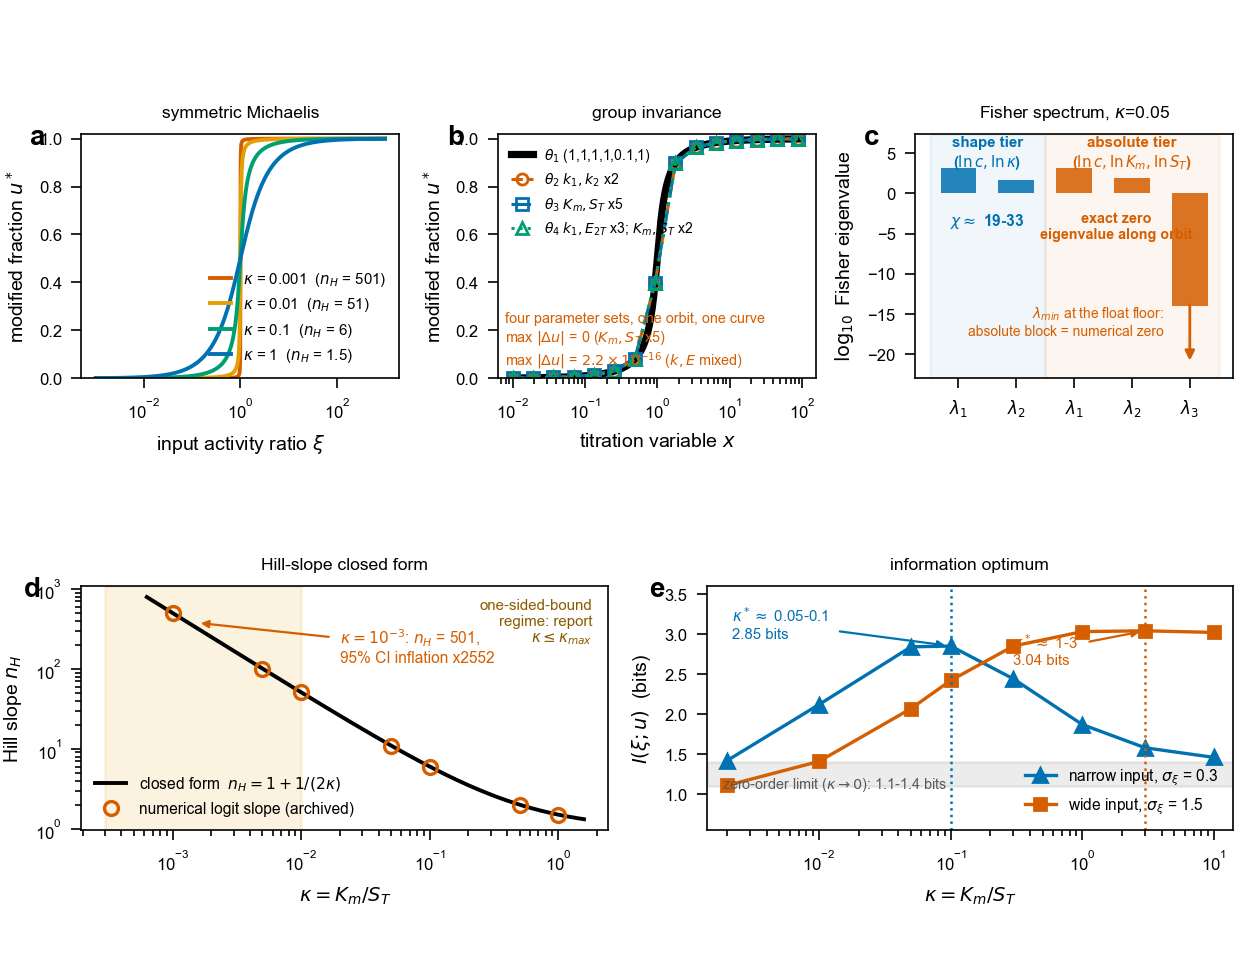
\includegraphics[width=\textwidth]{fig2_pdpc.png}
\caption{The static sensor. \textbf{a}, Steady-state curve family of Eq.~(\ref{eq:gk}); the Hill coefficient follows the closed form $n_H=1+1/(2\kappa)$. \textbf{b}, Degeneracy-group invariance: four parameter sets on one orbit produce one curve (max $|\Delta u|=0$ for the pure $(K_m,S_T)$ and rate rescalings; $2.2\times10^{-16}$ for the mixed rate--enzyme action). \textbf{c}, Fisher eigenspectrum at $\kappa=0.05$: the shape tier is well conditioned while the absolute tier carries an exact zero eigenvalue along the group orbit. \textbf{d}, The closed-form Hill slope against numerical logit slopes; in the deep zero-order region only a one-sided bound on $\kappa$ is reportable. \textbf{e}, Steady-state mutual information between a log-normal input ensemble and the noisy output has an interior optimum in $\kappa$; the zero-order limit is information-poor for all input widths.}
\label{fig:pdpc}
\end{figure}

\begin{figure}[p]
\centering
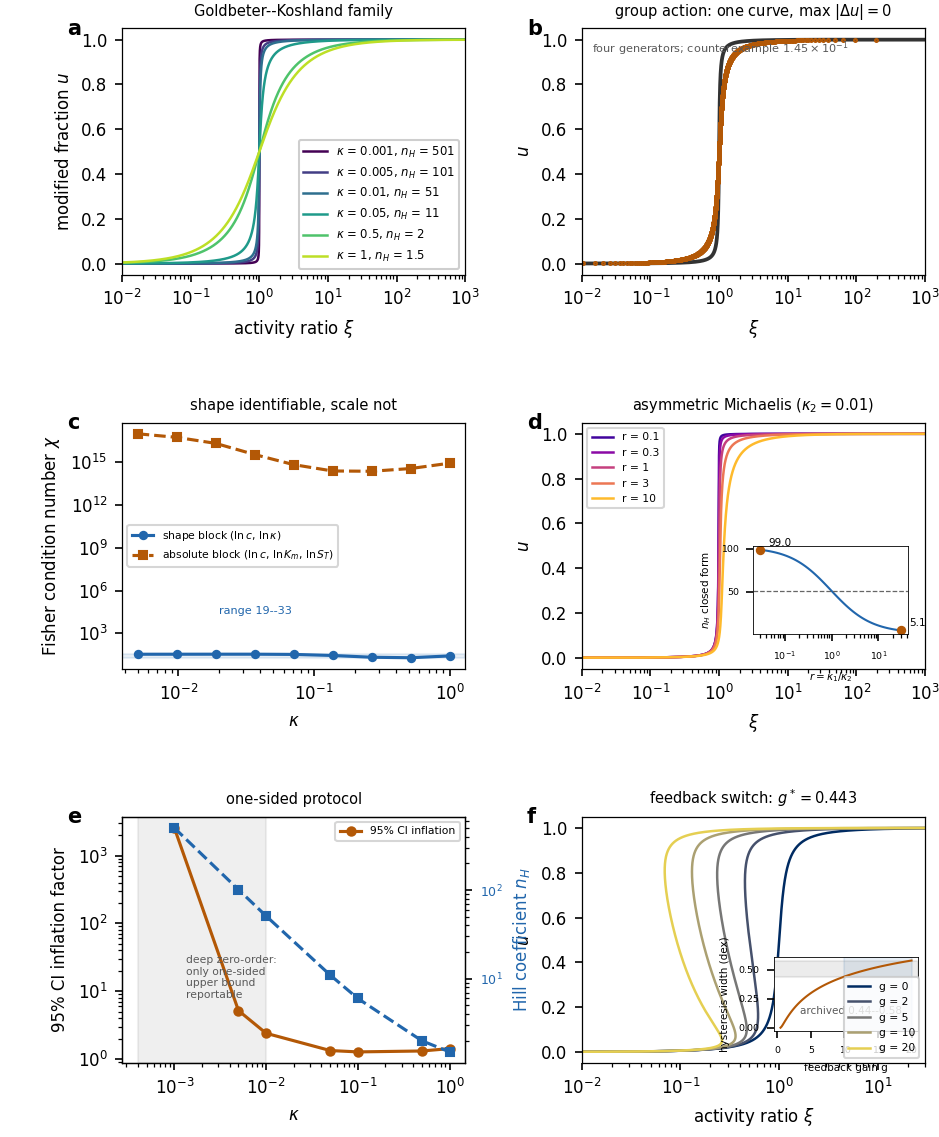
\includegraphics[width=\textwidth]{fig3_pdpc_full.png}
\caption{Extended analysis of the covalent cycle. \textbf{a}, Goldbeter--Koshland curve family across $\kappa$. \textbf{b}, The four group generators verified to machine precision, with a counterexample action moving the curve by $1.45\times10^{-1}$. \textbf{c}, Fisher condition numbers: the shape block stays at $\chi\approx19$--$33$ while the absolute block retains a numerical-zero eigenvalue at every $\kappa$. \textbf{d}, Asymmetric-Michaelis curves; inset, the closed form of Eq.~(\ref{eq:hill}) against the asymmetry ratio. \textbf{e}, Confidence-width inflation along the saturation axis (Table~\ref{tab:onesided}); below $\kappa\lesssim0.01$ only a one-sided upper bound is reportable. \textbf{f}, The positive-feedback switch: beyond $g^*=0.443$ the response folds, the apparent Hill coefficient rises steeply with feedback gain, and every bistable branch remains group-invariant.}
\label{fig:pdpcfull}
\end{figure}

\section{Worked instance 2: the morphogen anchor is absolute and free}
\label{sec:bicoid}

The Drosophila blastoderm is the strongest candidate counterexample to the free-first principle: gap-gene boundaries are read at fractional positions $x/L$, and embryos vary in length. If the positional readout required a maintained absolute ruler, a paid reference would have to sit somewhere in the axis. The record shows the opposite division of labour: the anchor is absolute but supplied free by physics, and the scaling of the readout is supplied by a geometric counter.

We re-analysed the per-boundary precision and scaling tables of Morton de Lachapelle and Bergmann \cite{Bergmann2010} (84 boundaries across Kr, Gt, Hb and Eve stripes 1--7 at $1\times$, $2\times$ and $4\times$ bcd dosage, more than 150 embryos) and the per-embryo Bicoid profiles of Liu et al.\ \cite{Liu2013} distributed by Nikoli\'c et al.\ \cite{Nikolic2023} (581 embryos passing quality control). Four checks were specified before the scaling table was opened; three are met as stated and one only in its direction (Fig.~\ref{fig:instances}a). Anterior hyper-scaling: at $1\times$ dosage the ten boundaries anterior to 35\% embryo length have median $S=1.728$ (range 1.59--2.04), all ten point estimates above unity, and 5 of the 10 with the 68\% confidence interval excluding unity. Mid-embryo near-perfect scaling (35--70\% embryo length): median $S=1.175$ at $1\times$ and $1.067$ at $2\times$, with 53\% (8/15) and 59\% (10/17) of boundaries consistent with $S=1$ within the 68\% interval. Monotone dose dependence: the confidence-weighted mean $S$ falls $1.069\to0.955\to0.841$ as bcd dosage rises $1\times\to2\times\to4\times$, and at $4\times$ the mid-embryo domain turns hypo-scaling (median 0.782; 0 of 22 with the 68\% interval excluding unity). Precision does not collapse posteriorly: $\sigma(x/L)$ median 2.11\% of embryo length over all 84 boundaries (range 0.93--4.09\%).

The dose dependence of $S$ is the signature of threshold-crossing readout: boundary positions are read off the Bcd concentration profile, so the scaling coefficient inherits the profile's own scaling. Among the four candidate mechanisms compared in the source study, the observed $S(x)$ shape (anterior hyper-scaling, mid-embryo near-perfect scaling, mild posterior hypo-scaling (median $S=0.889$ over the 36 boundaries posterior to 56\% embryo length)) selects the nuclear-density degradation model, in which Bcd degradation tracks nuclear density $\propto N/L^2$ as nuclei divide. Nuclear density is a geometric counting object: counting nuclei measures embryo length without any maintained reference, so length normalisation comes free with development.

The anchor side was tested per embryo in absolute coordinates. Exponential length constants fitted embryo by embryo ($x=x_s\cdot L$, window $x/L\in[0.10,0.50]$, median fit $R^2=0.985$) give the scaling exponent of the length constant, $\lambda\propto L^{\alpha}$, as
\begin{equation}
\alpha=-0.182,\qquad 95\%\ \mathrm{CI}\ [-0.476,\,+0.109]\quad(581\ \text{embryos, bootstrap}\times2000),
\label{eq:alpha}
\end{equation}
against frozen lines (anchor: point $\le0.7$ with CI upper below 1; perfect scaling: point $\ge0.9$). Exact scaling ($\alpha=1$) is excluded at $8.3\sigma$ and the frozen $0.9$ decision line at $7.6\sigma$; the median $\lambda=87.6\ \mu$m sits in the literature band 80--100 $\mu$m, a pipeline-correctness control. The length constant is absolute within the species because it is fixed by diffusion and degradation constants, which are class-II objects maintained by physics: natural $\pm10\%$ length variation is absorbed without retuning.

Two cross-regime consistencies, recorded as post hoc and not counted toward the score, close the loop. Across species, the per-species distributions of $\lambda/L$ (27 \emph{L.\ sericata}, 35 \emph{D.\ melanogaster}, 18 \emph{D.\ busckii} embryos \cite{Gregor2005}) have means agreeing within 2\% under a fixed nuclear count ($\log_2 N_{\mathrm{nuc}}=12.8\pm0.2$), and the inferred lifetime retuning (about 3 min in \emph{D.\ busckii} to 32 min in \emph{L.\ sericata}) is supplied by counting geometry rather than per-species molecular recalibration. Within species, on the size-selected inbred lines of Cheung et al.\ \cite{Cheung2014} ($L$ ratio $1.236\pm0.068$), the nuclear-density prediction $\lambda\propto L$ gives 126.8 $\mu$m against the observed $141.8\pm19.1\ \mu$m ($0.78\sigma$), with the residual in the direction of the documented confound in that line (an abnormally broadened bcd mRNA source). The two regimes are one statement: molecular constants are fixed; what rescales the anchor across size regimes is nuclear-counting geometry, a class-I carrier.

Two tensions are registered rather than resolved. Cross-species $\lambda\propto L$ over a five-fold length range \cite{Gregor2005} and partial within-species retuning in abnormally large embryos ($\lambda$ 102.6 to 141.8 $\mu$m \cite{Liu2013,Cheung2014}) define a two-regime picture whose quantitative boundary needs the large-embryo per-embryo data, which are not publicly available; the existing per-embryo resources \cite{Gregor2007,Petkova2019} cover wild-type-sized embryos. And the framework reading of the two maternal systems (anterior bcd mRNA anchoring and the terminal Torso system as the axis's paid references) is falsifiable: disruption of the anterior anchoring machinery (the exu/swa class) is predicted to move the anterior scaling behaviour selectively, sparing the mid-embryo. Qualitative anterior deletions in those mutants are compatible; the scaling-signature test has not been performed.

\section{Worked instance 3: Wnt reads fold change on a quantised plateau}
\label{sec:wnt}

Goentoro and Kirschner reported that $\beta$-catenin signalling reads the fold change over background rather than the absolute level \cite{Goentoro2009Wnt}. The source study provides no machine-readable supplementary data, so we digitised its Fig.\ 4F (fold-change versus LiCl dose; two-point log-linear calibration; registered precision $\pm0.05$ relative fold-change, $\pm2$ mM) and scored two frozen checks (Fig.~\ref{fig:instances}b). Plateau: the four digitised points between 7 and 49 mM LiCl fall within $\pm5\%$ of unity (0.964, 1.040, 1.021, 0.983); the sub-7 mM range is unresolved, the lowest-dose entry being a merged cluster spanning 0--20 mM. Breakdown: fold change falls from 0.983 at 48.6 mM to 0.605 at 58.1 mM and to 0.25--0.27 at 70--82 mM, so the breakdown is bracketed between 48.6 and 58.1 mM, compatible within digitisation precision ($\pm2$ mM) with the original qualitative statement. Corroborating panels read at lower precision: Axin1 overexpression leaves fold change at $\approx1$, and 80 mM LiCl compresses the Wnt3a response fold change from $\approx6$ to $\approx1.5$.

The normalisation mechanism identified in the source literature, the balance of synthesis and destruction-complex turnover, is a synthesis--degradation ratio of class-I type and requires no maintained paid reference. Wnt/$\beta$-catenin is thereby the third system in the ratio-law camp alongside fold-change detection in gene regulation \cite{Goentoro2009iFFL,Shoval2010,Adler2018} and bacterial chemotaxis \cite{Lazova2011,Shimizu2010}. The instance carries one registered limitation (single source, single readout arm) and one frozen falsifiable prediction: overexpression of Axin, which enlarges the destruction-complex capacity, is predicted to move the breakdown boundary (48.6--58.1 mM LiCl) to higher doses, with the shift estimable from the destruction-complex turnover ratio.

\section{Worked instance 4: cascades kill amplitude in the gain distribution}
\label{sec:cascade}

The instances above treat each system at a single level. The cascade question is what survives a relay.

\textbf{The M3R-to-Ca$^{2+}$ two-stage cascade.} Keshelava et al.\ \cite{Keshelava2018} recorded per-cell Fura-2 peaks for 433 cells stimulated at seven acetylcholine concentrations with five repetitions, across 27 experiments; 353 cells with complete $7\times5$ matrices entered analysis. The population dose--response drifts hard: per-experiment Hill fits give a median EC$_{50}$ of $0.63\ \mu$M with CV 1.16 and a 32-fold range (0.16--5.17 $\mu$M, no bound collisions). The single cell underneath is precise: median within-cell CV across the five identical repetitions is 3.4--3.7\% at the two highest doses, and per-cell rank is preserved across adjacent doses (Spearman $\rho=0.90, 0.86, 0.85, 0.87, 0.73, 0.58$ descending the ladder), while the across-cell CV of the per-cell mean is 28--36\% at high dose and exceeds 50\% at low dose (Fig.~\ref{fig:instances}c). Adjacent-dose discrimination from raw amplitude gives AUC 0.556--0.733; self-normalisation to each cell's own maximal-dose response gives no significant improvement (0.547--0.735), a negative result whose interpretation is registered: the five-repetition averaging already compresses within-cell noise to 3.5\%, so the decoding bottleneck is the across-cell gain distribution, not intracellular noise. At the low-dose end, dose information is carried by whether the cell responds at all (responding fraction $1.00\to0.24$ over the ladder). Because a cell cannot know its own position in the across-cell gain distribution, absolute amplitude is not a reportable statistic downstream of the first stage; self-referenced statistics and event presence are what survive.

\textbf{The chemotaxis three-stage relay.} In the bacterial chemotaxis chain, the receptor-cluster layer is where a model-class tension has been reported \cite{CompanionChemo}; that analysis is under revision and nothing below depends on its resolution. What the relay itself does is independent of it: across 2,217 cells and 77,595 pulse events from the Moore et al.\ archive \cite{Moore2024}, the pre-pulse baseline varies over only 0.056 activity units across previous-pulse doses from 0 to 180 $\mu$M, and the baseline difference between pulses following high and low predecessors is $-2.2\%$ of the median response amplitude. Baseline restoration is complete within the washout window and independent of dose history across a 90-fold range, the single-cell counterpart of robust perfect adaptation established as a design principle in \cite{Barkai1997,Yi2000}. The identified paid reference, the methylation-maintained effective affinity, sits at the relay that would have to absorb any upstream fracture.

\textbf{A falsified generalisation, recorded.} Whether the gain-distribution confinement generalises across pulse systems was tested under a frozen clause (confinement ratio $R\ge3$; falsification $R\le1.5$) on ERK-KTR pulse trains \cite{Chavez2022} and NF-$\kappa$B sequential-stimulation trains \cite{Wang2022}. Both clauses failed ($R=0.59$ and $1.08$; $R=1.20$, CI $[0.77,1.61]$), and the generalisation is withdrawn to the M3R case: amplitude in ERK/NF-$\kappa$B dies by within-cell pulse-to-pulse stochasticity rather than by across-cell gain dispersion. Both death modes deny amplitude an anchor, so the carrier-level conclusion is unchanged; the confinement mechanism is system-specific, and the falsification is registered with the same prominence as the confirmations (Table~\ref{tab:ledger}).

\textbf{Positive control: the class-III markers fire where they must.} A detector that never fires certifies nothing, so the three markers were applied to yeast osmotic homeostasis, where payment is functionally mandatory: cell volume and turgor are absolute quantities, the maintenance mechanism is identified (the Hog1--glycerol--Fps1 loop), and single-cell time courses with a causal inhibition arm are available \cite{Muzzey2009}. Marker 1, feedback on the reference itself: Hog1 activity returns to baseline (late-phase residual 2.55\% of peak) with perfect adaptation at all three shock doses, and recovery-phase correlation between Hog1 activity and volume is $r=-0.96$. Marker 2, recovery of the perturbed reference: 90\% recovery times are dose-ordered (11.0, 23.0, 28.0 min across the 0.2/0.4 M arms; the strong-shock 0.6 M arm, 59.0 min, listed separately under the frozen clause), with terminal values crossing the pre-shock baseline. Marker 3, continuously paid maintenance: internal glycerol is constant without shock while external glycerol accumulates monotonically when export is blocked, a synthesis--leakage equilibrium through Fps1. The deletion prediction P-1 fires causally on both sides of the loop: with Hog1 kinase chemically inhibited, absolute-scale volume recovery collapses from 0.644 to 0.070 (nine-fold separation) while the osmotic stimulus persists, and the signal itself stops adapting (late-phase residual 67\% of peak versus $-6.1\%$ uninhibited; Fig.~\ref{fig:instances}d).

\begin{figure}[p]
\centering
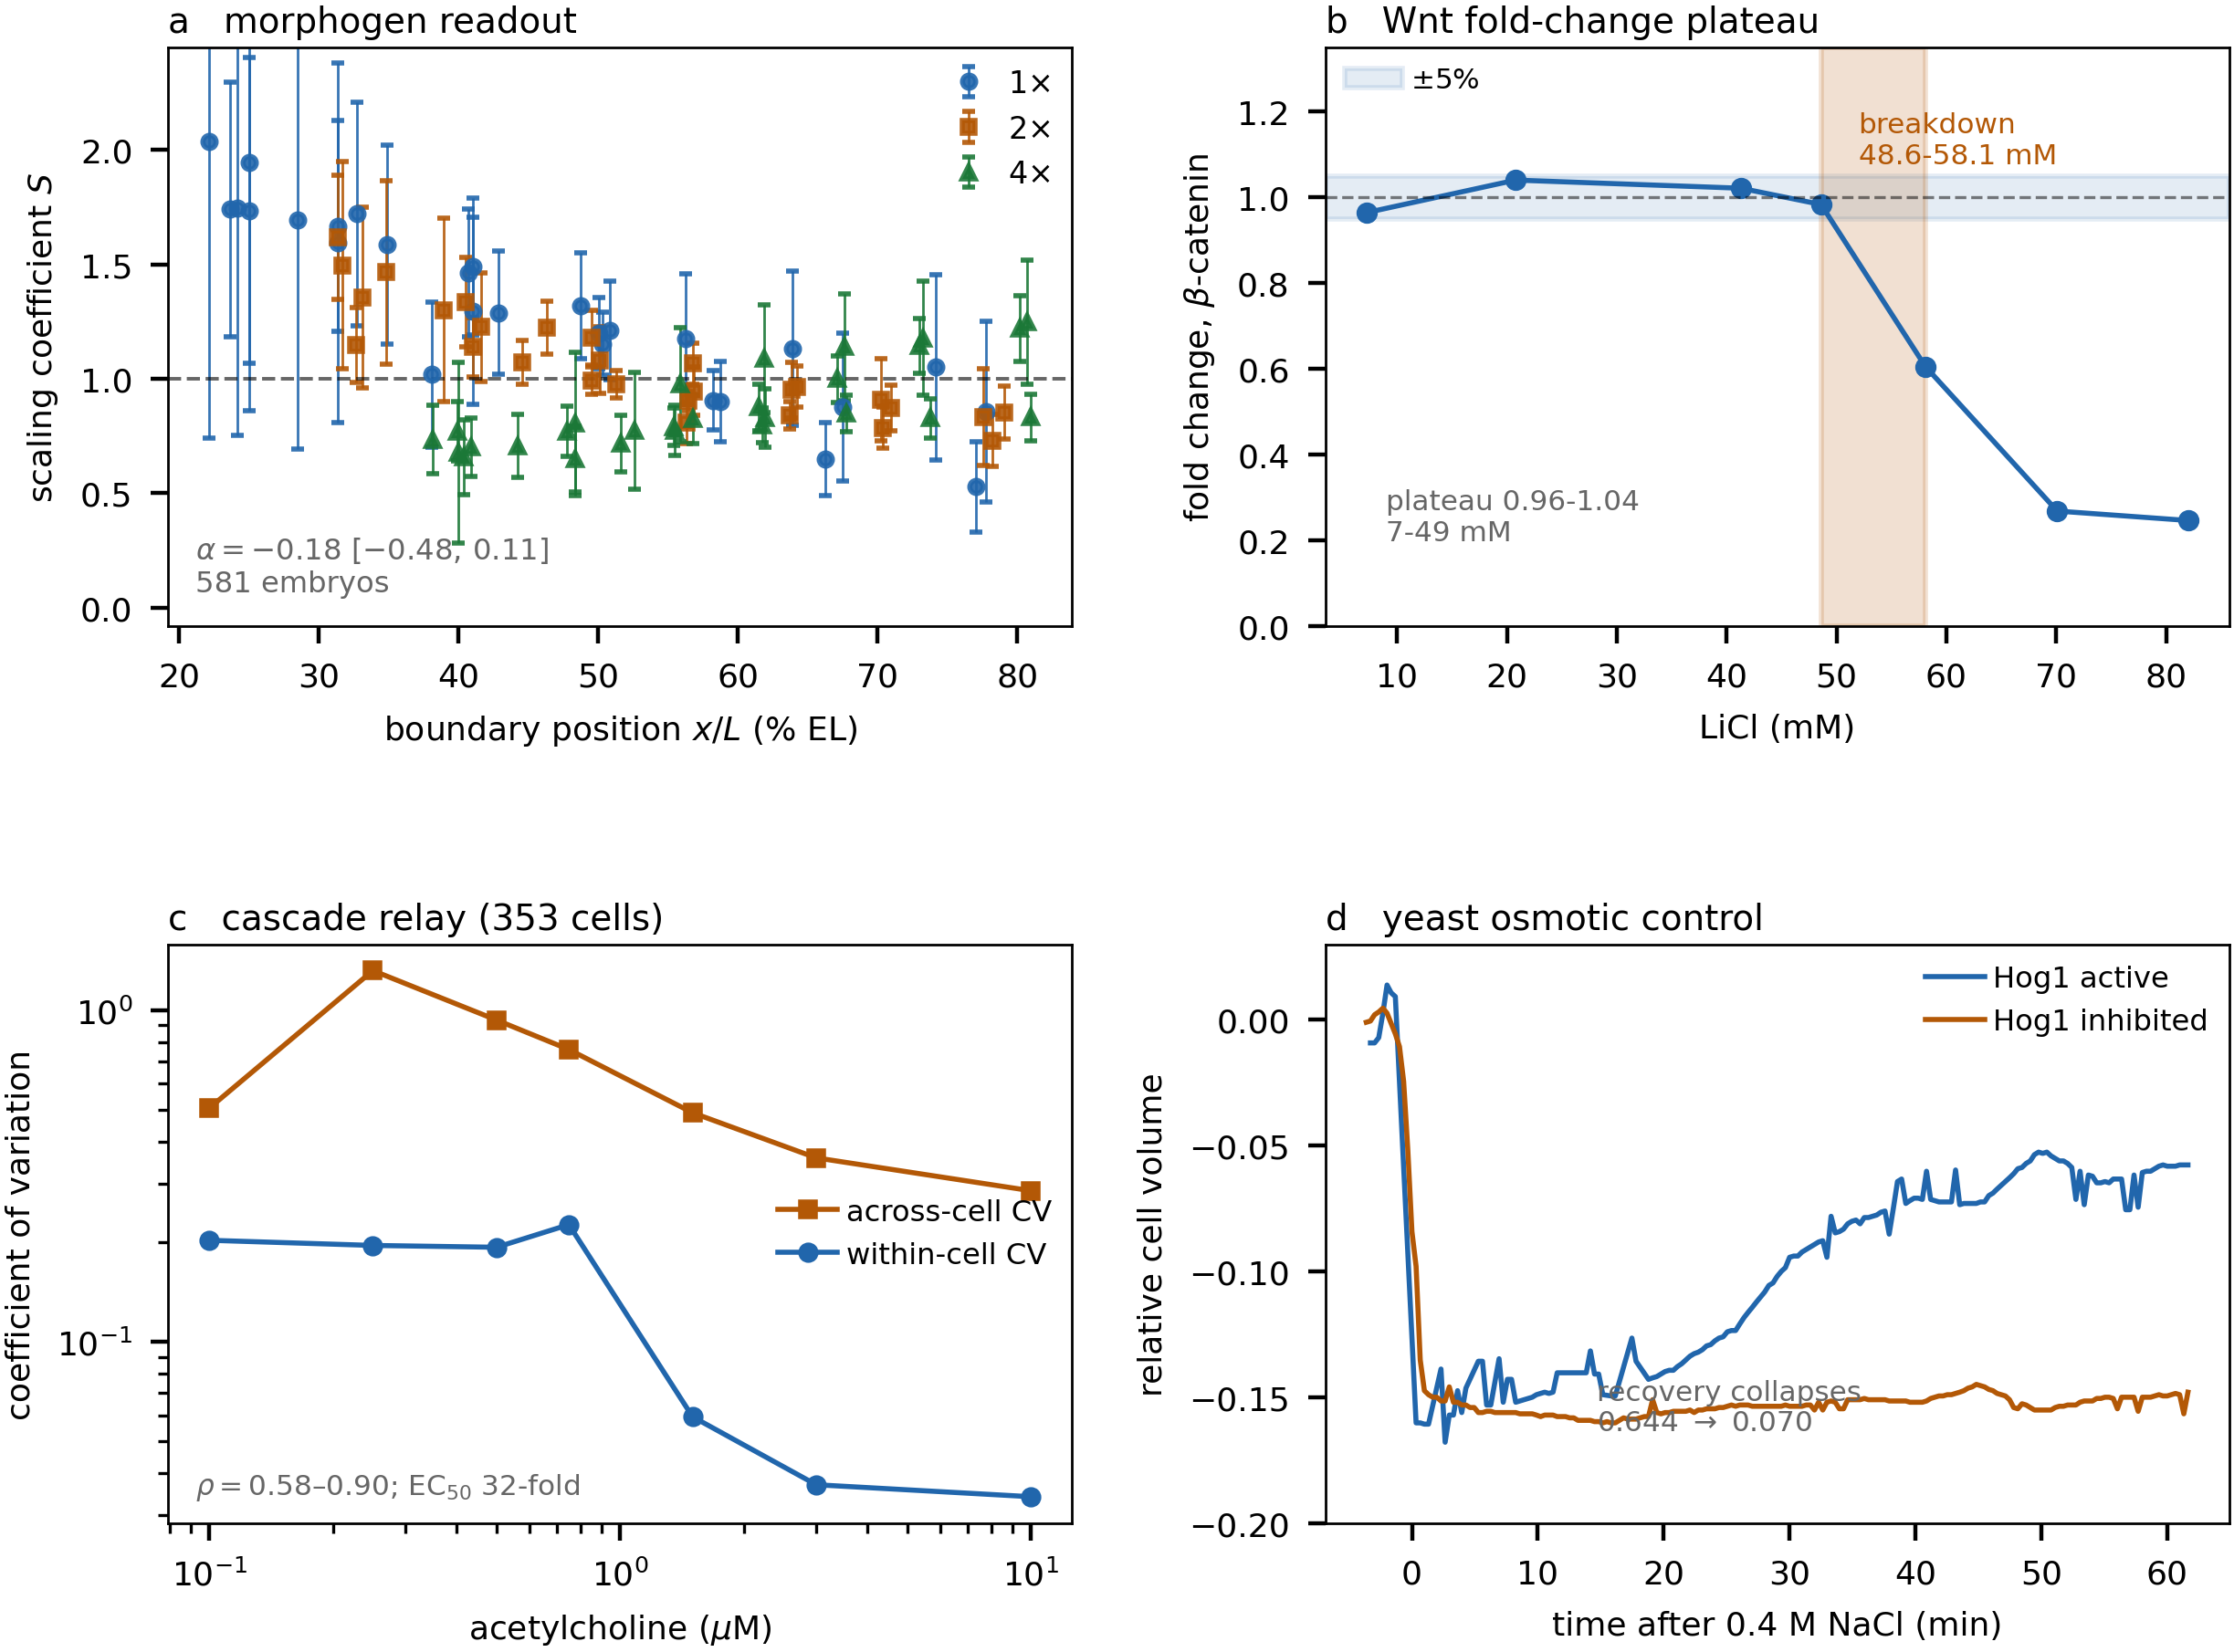
\includegraphics[width=\textwidth]{fig4_instances.png}
\caption{Four worked instances. \textbf{a}, Morphogen readout: per-boundary scaling coefficients of the gap-gene boundaries at three bcd dosages (84 boundaries; error bars, 68\% CI). Mid-embryo scaling is near 1 and falls monotonically with dose, the signature of threshold-crossing readout; the per-embryo anchor analysis gives $\alpha=-0.18$, excluding exact scaling at $8.3\sigma$. \textbf{b}, Wnt/$\beta$-catenin fold change versus LiCl dose (digitised from \cite{Goentoro2009Wnt}): plateau within $\pm5\%$ between 7 and 49 mM, breakdown bracketed between 48.6 and 58.1 mM. \textbf{c}, The M3R-to-Ca$^{2+}$ cascade: across-cell CV of the per-cell mean response dominates within-cell repeatability at every dose; per-cell rank is preserved ($\rho=0.58$--$0.90$) while across-experiment EC$_{50}$ values scatter over a 32-fold range. \textbf{d}, Positive control for class-III payment: yeast volume recovery after osmotic shock collapses from 0.644 to 0.070 when the Hog1 maintenance loop is inhibited.}
\label{fig:instances}
\end{figure}

\section{One census across systems}
\label{sec:census}

Table~\ref{tab:census} collects the carrier per system, including the three systems analysed at full depth in the companion papers \cite{CompanionP53,CompanionChemo,CompanionGPCR} and summarised here at one row each. The pattern is uniform in the rows that survived adjudication: wherever a calibration-free statistic suffices, it is the one used, and payment is concentrated at functionally necessary anchors. The ERK and NF-$\kappa$B carrier assignments are marked indeterminate because their blind adjudications did not confirm them. p53 counts dose while its amplitude is dose-invariant and functionally silent; NF-$\kappa$B and ERK digitise; Msn2 keeps frequency; chemotaxis reads fold change over two orders of magnitude of absolute ligand level while paying for one identified reference; the embryo reads relative position off an absolute anchor supplied free by physics; and where absolute scale is genuinely required, as in yeast volume homeostasis, all three class-III markers fire and causal inhibition of maintenance abolishes the absolute-scale function. The GPCR field row is the negative control at field level: no carrier is portable across laboratories, and the parameters drift unchecked.

\begin{table}[t]
\centering
\caption{The currency per system. Companion-paper rows are one-line summaries of \cite{CompanionP53,CompanionChemo,CompanionGPCR}; the remaining rows are this paper's worked instances. Class I: calibration-free statistics; class III: actively maintained paid references; a dash marks a carrier whose blind adjudication did not confirm it.}
\label{tab:census}
\small
\begin{tabular}{@{}p{3.2cm}p{4.4cm}p{1.5cm}p{5.2cm}@{}}
\toprule
\textbf{System} & \textbf{Carrier statistic} & \textbf{Class} & \textbf{Paid reference} \\
\midrule
p53, DSB response \cite{CompanionP53} & pulse count and timing; amplitude dose-invariant & I & none detected; noise scale is a Fisher null direction \\
NF-$\kappa$B \cite{Hoffmann2002,Tay2010} & not established: fold-change attribution intermediate ($R^2_{\rm fold}=0.006$ vs $0.008$, 18 units) & --- & none detected \\
ERK \cite{Albeck2013,Chavez2022} & event presence at the low-dose end only; trajectory decoding below line & --- & none detected \\
Msn2 \cite{Cai2008,Hao2012,Hansen2021} & event frequency & I & none \\
Bacterial chemotaxis \cite{CompanionChemo} & Weber fold change $\Delta L/L$ & I (readout) & methylation-maintained effective $K_d$ (class III) \\
GPCR pharmacology, field level \cite{CompanionGPCR} & none portable across laboratories & negative result & parameters drift unchecked \\
PdPC static sensor (this work) & ratio and threshold; $g^*=0.443$ & I & none \\
Bicoid to gap genes (this work) & relative position $x/L$ off threshold crossings & I (readout) & scaling paid by nuclear-density counting, a geometric counter; terminal anchors not tested (the scaling-signature test has not been performed) \\
Wnt/$\beta$-catenin (this work) & fold change over background; plateau within $\pm5\%$ between 7 and 49 mM LiCl & I & synthesis--degradation ratio of the destruction complex (no maintained reference) \\
Yeast osmotic homeostasis (positive control) & absolute volume and turgor & III & internal glycerol set point held by the Hog1--glycerol--Fps1 loop; all three markers fire; inhibition abolishes recovery ($0.644\to0.070$) \\
\bottomrule
\end{tabular}
\end{table}

\section{The prediction record}
\label{sec:ledger}

Every claim above was frozen in writing, with its verdict line, before the corresponding data values were inspected, and every outcome, including the falsifications, is recorded in the same ledger (Table~\ref{tab:ledger}; Fig.~\ref{fig:ledger}). The record across sixteen clauses is eight confirmations (four of them with registered contractions or corrections), six falsifications, and two clauses awaiting data. Two of the falsifications sharpened the claim by contraction: the gain-confinement rule now applies to the M3R cascade only, and the p53 counting law now applies inside the oscillatory regime only. Two literature-level consistencies were added post hoc and are labelled as such, not counted toward the score: the cross-species constancy of $\lambda/L$ under fixed nuclear count \cite{Gregor2005}, and the twelve-cell-line invariance of the p53 period near 5 h with all variation confined to envelope properties \cite{StewartOrnstein2017}.

\begin{figure}[p]
\centering
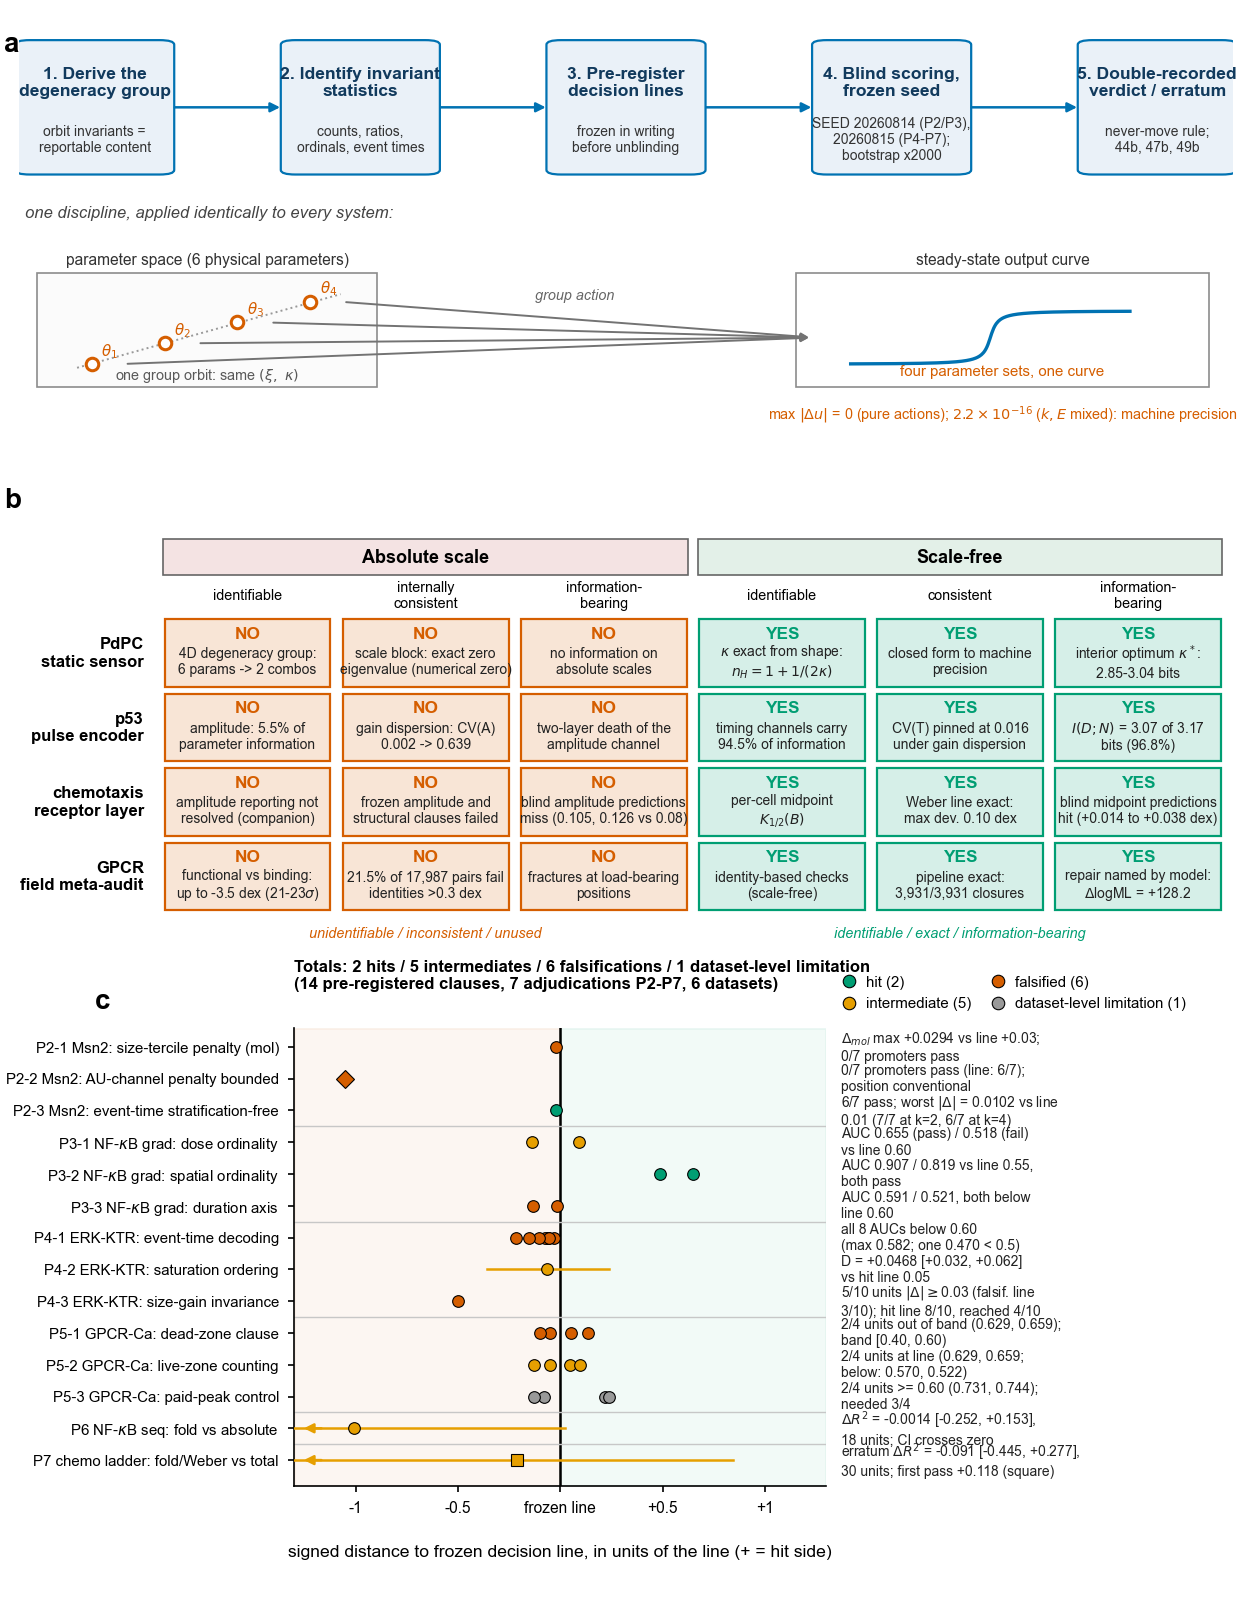
\includegraphics[width=\textwidth]{fig5_ledger.png}
\caption{One pattern, one record. \textbf{a}, The analysis discipline applied identically to every system: derive the degeneracy group, identify the invariant statistics, freeze the decision lines, score blind, and record failures twice; below, the group action collapses parameter space onto one curve. \textbf{b}, The stratification across the four deeply analysed systems (rows; companion papers \cite{CompanionP53,CompanionChemo,CompanionGPCR}): absolute-scale quantities are unidentifiable, internally inconsistent, or unreliable, while scale-free statistics are identifiable, exact, and information-bearing. \textbf{c}, The frozen-clause record of the blind adjudications: signed distance to each frozen decision line, in units of the line; hits, intermediates, falsifications and dataset-level limitations are plotted with the same prominence.}
\label{fig:ledger}
\end{figure}

\begin{table}[!tbp]
\centering
\caption{The prediction ledger: the win--loss record of the frozen prediction campaign. Falsifications are listed with the same prominence as confirmations; each falsification contracted the claim to what survived.}
\label{tab:ledger}
\scriptsize
\begin{tabular}{@{}p{5.4cm}p{4.0cm}p{3.0cm}@{}}
\toprule
\textbf{Frozen prediction} & \textbf{Outcome} & \textbf{Status} \\
\midrule
Bcd length constant is an absolute anchor & $\alpha=-0.18$, CI $[-0.48,0.11]$, 581 embryos; exact scaling excluded at $8.3\sigma$ & Confirmed \\
Gap-gene readout tracks relative position & mid-embryo median $S=1.175$ at $1\times$; dose-monotone $1.07,0.96,0.84$ & Confirmed \\
Wnt reads fold change with a quantised breakdown point & plateau 0.96--1.04 at 7--49 mM; breakdown 48.6--58.1 mM & Confirmed \\
Chemotaxis mixed-ligand midpoints (prospective, blind) & $+0.014$, $+0.038\dex$ inside band; the other two clauses of the same battery failed & Confirmed for midpoints only \\
p53 dose is encoded in pulse count, not amplitude & timing share 94.5\% at the representative calibration; reverses at mechanism level (45.1\% against 54.9\%) & Confirmed at representative level \\
Oncogenic Ras/Raf compress ligand-to-ERK channel capacity & G12D $-0.228$, Q61R $-0.335$, BRAF-V600E $-0.413$ bits; graded with allele strength & Confirmed for strong alleles \\
Downstream decoders misread the p53 regime switch & 29.0\% of induced genes $>2\times$ higher under sustained p53; 11.1\% reverse; 49.3\% within $2\times$ & Confirmed with correction \\
Resistance mutations preserve catalytic activity & ABL Y253H 2.46-fold, E255V 1.73-fold vs WT; EGFR resistance variants retain activity & Confirmed; manifold split \\
Gain-confinement generalises across pulse systems & $R=0.59$--$2.17$; line not met in ERK or NF-$\kappa$B & Falsified; contracted to M3R \\
Amplitude stratification (Msn2); duration axis (NF-$\kappa$B); event time (ERK-KTR) & Msn2 amplitude and ERK event-time failed; NF-$\kappa$B intermediate & Falsified for two, intermediate for one \\
Size--gain operationalisation of cheapest-sufficient-invariance & relation absent & Falsified; clause contracted \\
Slow DNA repair yields more p53 pulses at fixed dose & $\rho=+0.857$, direction reversed; repair failure switches to a sustained regime & Falsified; counting law contracted \\
Oncogenic alleles widen the across-cell ERK gain distribution & $|\Delta\mathrm{CV}|\le0.014$ across isogenic lines & Falsified \\
Tissue-level pERK decouples from receptor abundance in mutant tumours & WT coupling present in LUAD ($-0.25$, $p=0.006$), absent in COADREAD; mutants steeper, not absent & Falsified at bulk resolution \\
KRAS-G13D channel capacity intermediate between G12V and G12D & no comparable public dataset as of writing & Awaiting test \\
Zero hysteresis in the p53 dose response under a two-way scan & experiment never performed; protocol frozen with decision criteria \cite{CompanionP53} & Awaiting test \\
\bottomrule
\end{tabular}
\end{table}

\section{Discussion}

\textbf{The gauge principle.} Because observables depend only on dimensionless combinations, the functionally complete description of a circuit lives in dimensionless coordinates; absolute molecular scales are a redundant gauge. Three practices follow. Experimentally, perturbations and cross-system comparisons are meaningful only when stated on dimensionless groups: comparing absolute rate constants across cell types conflates gauge with physics. Evolutionarily, mutation walks in absolute coordinates while selection reads dimensionless ones, so the degeneracy group is the neutral-drift space available to a circuit, which formalises how molecular degeneracy supports resilience \cite{Prinz2004,Goaillard2021}. Functionally, the principle rationalises why biological sensing is so often ratio-based \cite{Goentoro2009iFFL,Adler2018,Bergmann2010}: a cell has no external calibration standard, so evolution can only have built its sensors on dimensionless quantities. Counting is the limiting case in which the observable is dimensionless by construction \cite{Vogelstein1999,Guo2026}, the measurement-theoretic endpoint \cite{Krantz1971} that rate-independent chemical computation reaches from the engineering side \cite{Chen2023}.

\textbf{The free-first principle and its falsifier.} The record assembled here supports the cost-effectiveness reading: wherever a calibration-free statistic suffices for the function, it is the one used, and payment for an actively maintained reference occurs exactly where function must reference absolute scale. The principle is not an optimality claim about evolution in general; it is a statement about which carrier a function can use at all, given the gauge freedom of the intracellular environment. Its falsifier is explicit: a single position whose function references only relative quantities yet hosts an active, energy-consuming reference-maintenance mechanism. The positive control shows the markers can fire; the morphogen instance shows the complementary direction, an absolute anchor that is free because physics supplies it. We regard the principle as the component of this work most exposed to future data, and the exposure is deliberate.

\textbf{What this study adds.} Nondimensionalisation, degeneracy groups, Fisher stratification, scan-based one-sided bounds and orthogonal experimental design each have decades of precedent, and we claim no methodological novelty. The novelty is of application and output: a computable survival set with sharp algebraic content for the generic interface; an exact degeneracy group with reporting protocols for a core signalling circuit; a three-class reference taxonomy whose markers are scored independently of the framework's predictions; and four worked instances in which the economics of absolute scale are measured rather than asserted, including one instance (the morphogen axis) where the framework survived its most dangerous test, an absolute positional coordinate that turned out to be supplied free by physics and counting geometry. On the assay side of the measurement boundary, the same law has been found independently: platforms count when they cannot calibrate \cite{Guo2026,Vogelstein1999}. Cells, the original uncalibratable instruments, do the same.

\textbf{Boundaries.} Seven considerations bound the claims. (1) Analogue information is not excluded in principle: where cells report graded quantities, the payment rule predicts the calibration cost is paid explicitly, and morphogen biology reads as a catalogue of such payments. (2) Information statements concern steady-state, single-readout channels; the bounds describe what is robustly transferable per unit of calibration effort, not what is transferable in principle. (3) The survival set is defined relative to a noise-calibrated threshold, so borderline statistics can shift class with measurement quality. (4) The class-III signature is a forward search instruction, not an executable reverse falsification: an exhaustive search finding no maintenance triggers re-examination, not a verdict against the framework. (5) The worked instances re-analyse public data; the Wnt instance and the yeast glycerol arms rest on digitised figures at registered digitisation-level precision, sufficient for plateau and collapse claims but not for sub-10\% statements. (6) The morphogen instance carries two registered tensions (cross-species scaling and large-embryo retuning) whose resolution requires per-embryo data that are not public. (7) The census covers the systems we have analysed; it is not a sample of all signalling, and the falsifier of the free-first principle may live in a system not yet examined.

\textbf{Outlook.} The framework's constructive content, what a circuit must look like when the analogue scale factor cancels from its likelihood, is developed for the two circuit classes in the companion papers: the static cycle reaches the limit by chemical saturation and the pulse encoder by circuit topology, and both limits degenerate to counting statistics \cite{CompanionP53}. The reverse direction, reading cellular economics from artificial perception networks evolved under controlled perturbation regimes, produces candidate cross-domain laws whose cellular predictions are frozen and awaiting test. If the principle survives, it is a design rule: synthetic circuits that must transmit dose under unresolvable parameter uncertainty should be built to count.

\section{Methods}

\subsection{Formalism conventions and status of statements}

The layer model, degeneracy group (Eq.~\ref{eq:group}), survival set (Eq.~\ref{eq:survival}), three-leg criterion and reference taxonomy are as defined in Sections \ref{sec:model} and \ref{sec:payment}. Theorem 1 is a theorem given the model (telescoping plus data-processing inequality); Theorems 2--4 are proved by direct construction and verified numerically as stated. The survival-set total-variation threshold $\varepsilon$ is calibrated per system to the measurement noise floor. The interface-algebra statements of Section \ref{sec:algebra} are exact algebraic identities for the affine interface. Numerical self-checks of the three legs and the identity on minimal stochastic models, including the bit-exact closure of the identity on a three-layer pulse-cascade model ($H(S)=2.322=0.435+0.593+1.294$ bits), are archived with the code.

\subsection{PdPC numerics}

Steady states of Eq.~\ref{eq:gk} and its asymmetric and positive-feedback extensions were solved by Brent's method (xtol $10^{-14}$). Group actions were verified on 200-point logarithmic titration grids; Fisher matrices were computed from the analytic Jacobian under additive Gaussian noise ($\sigma=0.03$, 20 points over three decades). The one-sided bound of Theorem 4 is a property of the likelihood-equivalent curve family and was checked for optimiser invariance. Mutual information in Fig.~\ref{fig:pdpc}e used binned log-normal input ensembles; absolute bit values are binning-sensitive and the interior-optimum conclusion rests on the ordering, which is robust across bin counts.

\subsection{Morphogen data and analysis}

Per-boundary precision and scaling tables of Morton de Lachapelle and Bergmann \cite{Bergmann2010} (PMC2858443, supplementary Datasets S1 and S2; 84 boundaries across Kr, Gt, Hb and Eve stripes 1--7 at three bcd dosages) were retrieved from the publisher archive and parsed verbatim; row-level correspondence between the two tables was asserted before analysis. Per-embryo Bcd profiles of Liu et al.\ \cite{Liu2013} (2XA reference line) were taken from the repository of Nikoli\'c et al.\ \cite{Nikolic2023}. Length constants were fitted embryo by embryo in absolute coordinates (window $x/L\in[0.10,0.50]$, log-linear; 581 of 582 embryos valid; median $R^2=0.985$); the exponent in Eq.~\ref{eq:alpha} was estimated by embryo-level bootstrap ($\times2000$) with a Theil--Sen control arm ($-0.199$). Verdict lines were frozen before data values were inspected (anchor: point $\le0.7$ and CI upper below 1; perfect scaling: point $\ge0.9$).

\subsection{Wnt digitisation}

Fig.\ 4F of Goentoro and Kirschner \cite{Goentoro2009Wnt} (PMC2921914) was digitised from the publisher archive image (468$\times$599; panel upscaled $4\times$): green marker centroids were extracted programmatically and mapped through a two-point log-linear calibration (y: 1 and 0.1 gridlines; x: 0 and 80 mM ticks). Registered precision: $\pm0.05$ relative fold change, $\pm2$ mM; sufficient for plateau and breakdown claims, not for sub-10\% statements.

\subsection{Cascade and chemotaxis-relay data}

Supplementary Data 3 of Keshelava et al.\ \cite{Keshelava2018} (PMC5830429; per-cell Fura-2 ratio peaks, baseline-subtracted by the authors' pipeline) was parsed verbatim: 27 experiments, 433 cells each stimulated at seven acetylcholine concentrations with five repetitions; 353 cells with complete $7\times5$ matrices entered analysis. Row-to-dose mapping was verified empirically (population mean peak declines monotonically; last row at baseline; within-row repetitions drift upward, excluding an adaptation artefact). A provenance discrepancy is registered: the authors' MATLAB script carries a legacy dose ladder different from the Methods ladder; all statistics reported here except absolute EC$_{50}$ values are invariant under monotone relabelling. The Moore et al.\ FRET archive \cite{Moore2024} (Dryad doi:10.5061/dryad.nvx0k6dzz) stores per-cell data as 35 events of 20 samples; 2,217 cells and 77,595 pulse events passed structural checks; the stimulus channel is stored as unsigned 8-bit integers and the pipeline corrects the resulting wrap-around in naive differencing.

\subsection{Yeast osmotic positive control}

Per-time-point numerical data of Muzzey et al.\ \cite{Muzzey2009} were taken from the authors' supplementary numerical tables (Hog1 activity and cell volume under 0.2/0.4/0.6 M NaCl shock, and the Hog1-as + PP1 causal-inhibition arm), with the glycerol synthesis--leakage arms digitised from the publisher figures; all arms were scored against the frozen marker definitions of Section~\ref{sec:payment}. The shut-off-to-recovery lag (22.0 min versus 28.0 min, $\Delta t=6.0$ min) sits marginally outside the frozen 5 min simultaneity line and is registered as intermediate under the frozen clause; all other marker evidence is as reported in Section~\ref{sec:cascade}.

\subsection{Analysis discipline}

Every prediction reported here was frozen in writing, with its verdict line, before the corresponding data values were inspected; seeds were fixed (20260927 for the morphogen and cascade adjudications; bootstrap $\times2000$ unless stated); failures and corrections were double-recorded and are listed in the repository ledger. The discipline is not claimed as a virtue; it is the mechanism by which Table~\ref{tab:ledger} can list falsifications at all.

\subsection{Data and code availability}

No new experimental data were generated. All analysis scripts, digitised tables and frozen verdict cards are available at \url{https://github.com/lihuanlz/scale-free-framework}, archived at Zenodo (doi:10.5281/zenodo.23402838; umbrella edition: doi:10.5281/zenodo.23008824). The companion papers \cite{CompanionP53,CompanionChemo,CompanionGPCR} use their own split repositories under the same account.

\section*{Acknowledgements}

This work re-analyses public single-cell and pharmacological data, and we thank the teams who produced, curated and shared these records: A. Morton de Lachapelle and S. Bergmann for the per-boundary precision and scaling tables of the Drosophila gap-gene read-out; T. Gregor and colleagues, F. Liu and colleagues, and M. Nikoli\'c and colleagues for the per-embryo Bicoid profiles and the scale-invariance repository; L. Goentoro and M. W. Kirschner for the Wnt fold-change study; A. Keshelava, V. L. Katanaev and colleagues for the GPCR-to-Ca$^{2+}$ single-cell archive; J. P. Moore, K. Kamino, T. S. Shimizu, T. Emonet and colleagues for the chemotaxis FRET archive, released CC0; D. Muzzey, C. A. G\'omez-Uribe, J. T. Mettetal and A. van Oudenaarden for the yeast osmoregulation time courses; and G. Lahav, E. Batchelor, S. Tay, J. Albeck and colleagues for the live-cell records summarised from the companion papers.

\section*{Author contributions}

H.L. conceived the study, proved the theorem-level statements, wrote and validated the analysis code, performed the analysis, and wrote the paper.

\section*{Competing interests}

The author declares no competing interests.

\begin{thebibliography}{99}
\small

\bibitem{Guo2026}
Guo, L. et al. Scale degeneracy and its resolution: the route to calibration-free absolute quantification. Preprint at ChemRxiv \url{https://doi.org/10.26434/chemrxiv-2024-19rj6/v10} (2026).

\bibitem{Vogelstein1999}
Vogelstein, B. \& Kinzler, K. W. Digital PCR. \emph{Proc. Natl Acad. Sci. USA} \textbf{96}, 9236--9241 (1999). \url{https://doi.org/10.1073/pnas.96.16.9236}

\bibitem{CompanionP53}
Li, H. The p53 pulse encoder counts by topological necessity: theory, evidence, and the molecular origin of the 5.5-hour clock. Companion manuscript (2026).

\bibitem{CompanionChemo}
Li, H. Amplitude and midpoint statistics of the same chemotaxis cells demand incompatible receptor models. Companion manuscript (2026).

\bibitem{CompanionGPCR}
Li, H. The quantitative currency of GPCR bias signalling fails its own algebraic identities. Companion manuscript (2026).

\bibitem{Tkacik2025}
Tka\v{c}ik, G. \& ten Wolde, P. R. Information processing in biochemical networks. \emph{Annu. Rev. Biophys.} \textbf{54}, 249--274 (2025). \url{https://doi.org/10.1146/annurev-biophys-060524-102720}

\bibitem{Cheong2011}
Cheong, R., Rhee, A., Wang, C. J., Nemenman, I. \& Levchenko, A. Information transduction capacity of noisy biochemical signaling networks. \emph{Science} \textbf{334}, 354--358 (2011). \url{https://doi.org/10.1126/science.1204553}

\bibitem{Selimkhanov2014}
Selimkhanov, J. et al. Accurate information transmission through dynamic biochemical signaling networks. \emph{Science} \textbf{346}, 1370--1373 (2014). \url{https://doi.org/10.1126/science.1254933}

\bibitem{Bowsher2014}
Bowsher, C. G. \& Swain, P. S. Environmental sensing, information transfer, and cellular decision-making. \emph{Curr. Opin. Biotechnol.} \textbf{28}, 149--155 (2014). \url{https://doi.org/10.1016/j.copbio.2014.04.010}

\bibitem{Govern2014}
Govern, C. C. \& ten Wolde, P. R. Optimal resource allocation in cellular sensing systems. \emph{Proc. Natl Acad. Sci. USA} \textbf{111}, 17486--17491 (2014). \url{https://doi.org/10.1073/pnas.1411524111}

\bibitem{Gutenkunst2007}
Gutenkunst, R. N. et al. Universally sloppy parameter sensitivities in systems biology models. \emph{PLoS Comput. Biol.} \textbf{3}, e189 (2007). \url{https://doi.org/10.1371/journal.pcbi.0030189}

\bibitem{Prinz2004}
Prinz, A. A., Bucher, D. \& Marder, E. Similar network activity from disparate circuit parameters. \emph{Nat. Neurosci.} \textbf{7}, 1345--1352 (2004). \url{https://doi.org/10.1038/nn1352}

\bibitem{Goaillard2021}
Goaillard, J.-M. \& Marder, E. Ion channel degeneracy, variability, and covariation in neuron and circuit resilience. \emph{Annu. Rev. Neurosci.} \textbf{44}, 335--357 (2021). \url{https://doi.org/10.1146/annurev-neuro-092920-121538}

\bibitem{Goentoro2009iFFL}
Goentoro, L., Shoval, O., Kirschner, M. W. \& Alon, U. The incoherent feedforward loop can provide fold-change detection in gene regulation. \emph{Mol. Cell} \textbf{36}, 894--899 (2009). \url{https://doi.org/10.1016/j.molcel.2009.11.018}

\bibitem{Shoval2010}
Shoval, O. et al. Fold-change detection and scalar symmetry of sensory input fields. \emph{Proc. Natl Acad. Sci. USA} \textbf{107}, 15995--16000 (2010). \url{https://doi.org/10.1073/pnas.1002352107}

\bibitem{Adler2018}
Adler, M. \& Alon, U. Fold-change detection in biological systems. \emph{Curr. Opin. Syst. Biol.} \textbf{8}, 81--89 (2018). \url{https://doi.org/10.1016/j.coisb.2017.12.005}

\bibitem{Goldbeter1981}
Goldbeter, A. \& Koshland, D. E. An amplified sensitivity arising from covalent modification in biological systems. \emph{Proc. Natl Acad. Sci. USA} \textbf{78}, 6840--6844 (1981). \url{https://doi.org/10.1073/pnas.78.11.6840}

\bibitem{Bergmann2010}
Morton de Lachapelle, A. \& Bergmann, S. Precision and scaling in morphogen gradient read-out. \emph{Mol. Syst. Biol.} \textbf{6}, 351 (2010). \url{https://doi.org/10.1038/msb.2010.7}

\bibitem{Liu2013}
Liu, F., Morrison, A. H. \& Gregor, T. Dynamic interpretation of maternal inputs by the Drosophila segmentation gene network. \emph{Proc. Natl Acad. Sci. USA} \textbf{110}, 6724--6729 (2013). \url{https://doi.org/10.1073/pnas.1220912110}

\bibitem{Nikolic2023}
Nikoli\'c, M. et al. Scale invariance in early embryonic development. \emph{Proc. Natl Acad. Sci. USA} \textbf{121}, e2403265121 (2024). \url{https://doi.org/10.1073/pnas.2403265121}

\bibitem{Gregor2005}
Gregor, T., Bialek, W., de Ruyter van Steveninck, R. R., Tank, D. W. \& Wieschaus, E. F. Diffusion and scaling during early embryonic pattern formation. \emph{Proc. Natl Acad. Sci. USA} \textbf{102}, 18403--18407 (2005). \url{https://doi.org/10.1073/pnas.0509483102}

\bibitem{Gregor2007}
Gregor, T., Tank, D. W., Wieschaus, E. F. \& Bialek, W. Probing the limits to positional information. \emph{Cell} \textbf{130}, 153--164 (2007). \url{https://doi.org/10.1016/j.cell.2007.05.025}

\bibitem{Petkova2019}
Petkova, M. D., Tka\v{c}ik, G., Bialek, W., Wieschaus, E. F. \& Gregor, T. Optimal decoding of cellular identities in a genetic network. \emph{Cell} \textbf{176}, 844--855 (2019). \url{https://doi.org/10.1016/j.cell.2019.01.007}

\bibitem{Cheung2014}
Cheung, D., Miles, C., Kreitman, M. \& Ma, J. Adaptation of the length scale and amplitude of the Bicoid gradient profile to achieve robust patterning in abnormally large Drosophila melanogaster embryos. \emph{Development} \textbf{141}, 124--135 (2014). \url{https://doi.org/10.1242/dev.098640}

\bibitem{Goentoro2009Wnt}
Goentoro, L. \& Kirschner, M. W. Evidence that fold-change, and not absolute level, of $\beta$-catenin dictates Wnt signaling. \emph{Mol. Cell} \textbf{36}, 872--884 (2009). \url{https://doi.org/10.1016/j.molcel.2009.11.017}

\bibitem{Lazova2011}
Lazova, M. D., Ahmed, T., Bellomo, D., Stocker, R. \& Shimizu, T. S. Response rescaling in bacterial chemotaxis. \emph{Proc. Natl Acad. Sci. USA} \textbf{108}, 13870--13875 (2011). \url{https://doi.org/10.1073/pnas.1108608108}

\bibitem{Shimizu2010}
Shimizu, T. S., Tu, Y. \& Berg, H. C. A modular gradient-sensing network for chemotaxis in Escherichia coli revealed by responses to time-varying stimuli. \emph{Mol. Syst. Biol.} \textbf{6}, 382 (2010). \url{https://doi.org/10.1038/msb.2010.37}

\bibitem{Keshelava2018}
Keshelava, A. et al. High capacity in G protein-coupled receptor signaling. \emph{Nat. Commun.} \textbf{9}, 876 (2018). \url{https://doi.org/10.1038/s41467-018-02868-y}

\bibitem{Moore2024}
Moore, J. P., Kamino, K., Kottou, R., Shimizu, T. S. \& Emonet, T. Signal integration and adaptive sensory diversity tuning in Escherichia coli chemotaxis. \emph{Cell Syst.} \textbf{15}, 628--638 (2024). \url{https://doi.org/10.1016/j.cels.2024.06.003}

\bibitem{Chavez2022}
Chavez-Abiega, S., Gr\"onloh, M. L. B., Gadella, T. W. J., Bruggeman, F. J. \& Goedhart, J. Single-cell imaging of ERK and Akt activation dynamics and heterogeneity induced by G-protein-coupled receptors. \emph{J. Cell Sci.} \textbf{135}, jcs259685 (2022). \url{https://doi.org/10.1242/jcs.259685}

\bibitem{Wang2022}
Wang, A. G., Son, M., Kenna, E., Thom, N. \& Tay, S. NF-$\kappa$B memory coordinates transcriptional responses to dynamic inflammatory stimuli. \emph{Cell Rep.} \textbf{40}, 111159 (2022). \url{https://doi.org/10.1016/j.celrep.2022.111159}

\bibitem{Muzzey2009}
Muzzey, D., G\'omez-Uribe, C. A., Mettetal, J. T. \& van Oudenaarden, A. A systems-level analysis of perfect adaptation in yeast osmoregulation. \emph{Cell} \textbf{138}, 160--171 (2009). \url{https://doi.org/10.1016/j.cell.2009.04.047}

\bibitem{Hoffmann2002}
Hoffmann, A., Levchenko, A., Scott, M. L. \& Baltimore, D. The I$\kappa$B--NF-$\kappa$B signaling module: temporal control and selective gene activation. \emph{Science} \textbf{298}, 1241--1245 (2002). \url{https://doi.org/10.1126/science.1071914}

\bibitem{Tay2010}
Tay, S. et al. Single-cell NF-$\kappa$B dynamics reveal digital activation and analogue information processing. \emph{Nature} \textbf{466}, 267--271 (2010). \url{https://doi.org/10.1038/nature09145}

\bibitem{Albeck2013}
Albeck, J. G., Mills, G. B. \& Brugge, J. S. Frequency-modulated pulses of ERK activity transmit quantitative proliferation signals. \emph{Mol. Cell} \textbf{49}, 249--261 (2013). \url{https://doi.org/10.1016/j.molcel.2012.11.002}

\bibitem{Cai2008}
Cai, L., Dalal, C. K. \& Elowitz, M. B. Frequency-modulated nuclear localization bursts coordinate gene regulation. \emph{Nature} \textbf{455}, 485--490 (2008). \url{https://doi.org/10.1038/nature07292}

\bibitem{Hao2012}
Hao, N. \& O'Shea, E. K. Signal-dependent dynamics of transcription factor translocation controls gene expression. \emph{Nat. Struct. Mol. Biol.} \textbf{19}, 31--39 (2012). \url{https://doi.org/10.1038/nsmb.2192}

\bibitem{Hansen2021}
Hansen, A. S. \& Zechner, C. Promoters adopt distinct dynamic manifestations depending on transcription factor context. \emph{Mol. Syst. Biol.} \textbf{17}, e9821 (2021). \url{https://doi.org/10.15252/msb.20209821}

\bibitem{Batchelor2011}
Batchelor, E., Loewer, A., Mock, C. \& Lahav, G. Stimulus-dependent dynamics of p53 in single cells. \emph{Mol. Syst. Biol.} \textbf{7}, 488 (2011). \url{https://doi.org/10.1038/msb.2011.20}

\bibitem{StewartOrnstein2017}
Stewart-Ornstein, J. \& Lahav, G. p53 dynamics in response to DNA damage vary across cell lines and are shaped by efficiency of DNA repair and activity of the kinase ATM. \emph{Sci. Signal.} \textbf{10}, eaah6671 (2017). \url{https://doi.org/10.1126/scisignal.aah6671}

\bibitem{Barkai1997}
Barkai, N. \& Leibler, S. Robustness in simple biochemical networks. \emph{Nature} \textbf{387}, 913--917 (1997). \url{https://doi.org/10.1038/43199}

\bibitem{Yi2000}
Yi, T.-M., Huang, Y., Simon, M. I. \& Doyle, J. Robust perfect adaptation in bacterial chemotaxis through integral feedback control. \emph{Proc. Natl Acad. Sci. USA} \textbf{97}, 4649--4653 (2000). \url{https://doi.org/10.1073/pnas.97.9.4649}

\bibitem{Krantz1971}
Krantz, D. H., Luce, R. D., Suppes, P. \& Tversky, A. \emph{Foundations of Measurement}, Vol.~I (Academic Press, 1971).

\bibitem{Chen2023}
Chen, H.-L., Doty, D. \& Soloveichik, D. Rate-independent computation in continuous chemical reaction networks. \emph{J. ACM} \textbf{70}, Article 22 (2023). \url{https://doi.org/10.1145/3590776}

\end{thebibliography}

\end{document}
